\documentclass{beamer}
\usetheme{Warsaw}
%\usetheme{metropolis}
%\usepackage[spanish,activeacute]{babel}
\usepackage[utf8]{inputenc}
\usepackage{listings}
\usepackage{amsmath,amsfonts,amssymb}
\usepackage{adjustbox}
\usepackage{color}
\usepackage{tikz}
\usetikzlibrary{shapes,arrows}
\usepackage{multicol}
\usepackage{hhline}
\usepackage{pgf}
\usepackage{algorithm} 
\usepackage{algorithmic}
\renewcommand{\algorithmicrequire}{\textbf{Input:}}
\renewcommand{\algorithmicensure}{\textbf{Output:}}
\def\R{{\mathbb R }}
\def\N{{\mathbb N }}

   \definecolor{myblue1}{RGB}{35,119,189}
    \definecolor{myblue2}{RGB}{95,179,238}
    \definecolor{myblue3}{RGB}{129,168,207}
    \definecolor{myblue4}{RGB}{26,89,142}

    \setbeamercolor*{structure}{fg=myblue1,bg=blue}
    \setbeamercolor*{palette primary}{use=structure,fg=white,bg=structure.fg}
    \setbeamercolor*{palette secondary}{use=structure,fg=white,bg=structure.fg!75!black}
    \setbeamercolor*{palette tertiary}{use=structure,fg=white,bg=structure.fg!50!black}
    \setbeamercolor*{palette quaternary}{fg=black,bg=white}

    \setbeamercolor*{item projected}{fg=red,bg=myblue3!80}
    \setbeamercolor*{block title example}{fg=white,bg=myblue4}
    \setbeamercolor*{frametitle}{fg=black}

    \setbeamertemplate{blocks}[rounded][shadow=true]

    \makeatletter
    \pgfdeclarehorizontalshading[frametitle.bg,frametitle right.bg]{beamer@frametitleshade}{\paperheight}{%
      color(0pt)=(myblue2);
      color(\paperwidth)=(white)}

    \defbeamertemplate*{footline}{mysplit theme}
    {%
      \leavevmode%
      \hbox{\begin{beamercolorbox}[wd=.5\paperwidth,ht=2.5ex,dp=1.125ex,leftskip=.3cm plus1fill,rightskip=.3cm]{author in head/foot}%
        \usebeamerfont{author in head/foot}\insertshortauthor
      \end{beamercolorbox}%
      \begin{beamercolorbox}[wd=.5\paperwidth,ht=2.5ex,dp=1.125ex,leftskip=.3cm,rightskip=.3cm plus1fil]{title in head/foot}%
        \usebeamerfont{title in head/foot}\insertshorttitle\hfill
        \insertframenumber/\inserttotalframenumber\hspace*{0.5em}
      \end{beamercolorbox}}%
      \vskip0pt%
    }
    \makeatother


\author[Paola Arce]{Paola Arce \\ Departamento de Inform\'atica, UTFSM \\ Thesis advisor: Luis Salinas}
\date{December 15, 2017}
\title[Thesis defense]{Online learning methods for financial time series forecasting}
\subtitle{PhD Thesis Defense}

\titlegraphic{
    \tikz[overlay,remember picture]
        \node[at=(current page.south), anchor=south] {
            
\includegraphics[height=1.5cm]{img/DIT}
        };
}

\begin{document}
\begin{frame}[plain]
\titlepage
\end{frame}


\begin{frame}
\frametitle{Outline}
\begin{itemize}
\item Motivation: economic relations
\item Cointegration and Integration concepts
\item VECM model
\item Proposal
\item Experiments
\item Conclusions
\end{itemize}
\end{frame}

\section{Introduction}

\begin{frame}
\frametitle{Motivation}
Most financial time series are non-stationary in nature. This implies that the statistical properties, such as mean and variance of the data change over time. Therefore, financial time series forecasting is still a challenge.
\begin{figure}
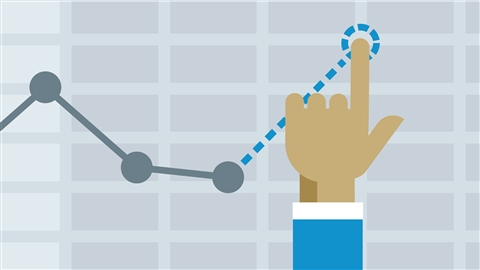
\includegraphics[width=0.4\paperwidth]{img/forecast}
\end{figure}

\end{frame}

\begin{frame}
\hspace*{-4mm}
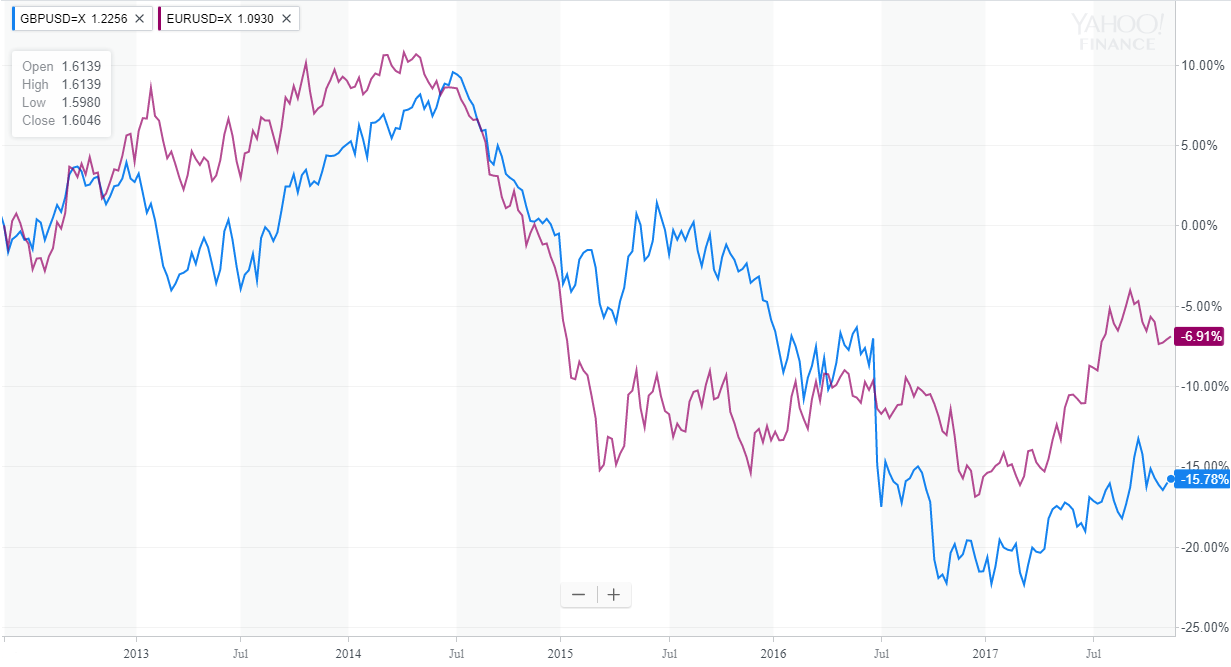
\includegraphics[width=0.9\paperwidth]{img/motivation.png}
\end{frame}

\begin{frame}[t,fragile]{Random walk and Cointegration Illustration}
 \begin{itemize}
  \item<1-> The drunkard's walk
  \item<2-> The dog's walk
  %\item<3-> The drunk and dog's walk
 \end{itemize}
 
\begin{columns}
\begin{column}{.4\linewidth}<1->
\begin{center}
        \begin{tikzpicture}[overlay]
            \node[yshift=-50] (img2) {
\includegraphics[scale=1.4]{img/drunk}};
        \end{tikzpicture}
\end{center}
\end{column}
\begin{column}{.08\linewidth}<2->
        \begin{tikzpicture}[overlay]
            \node[yshift=-50] (img2) {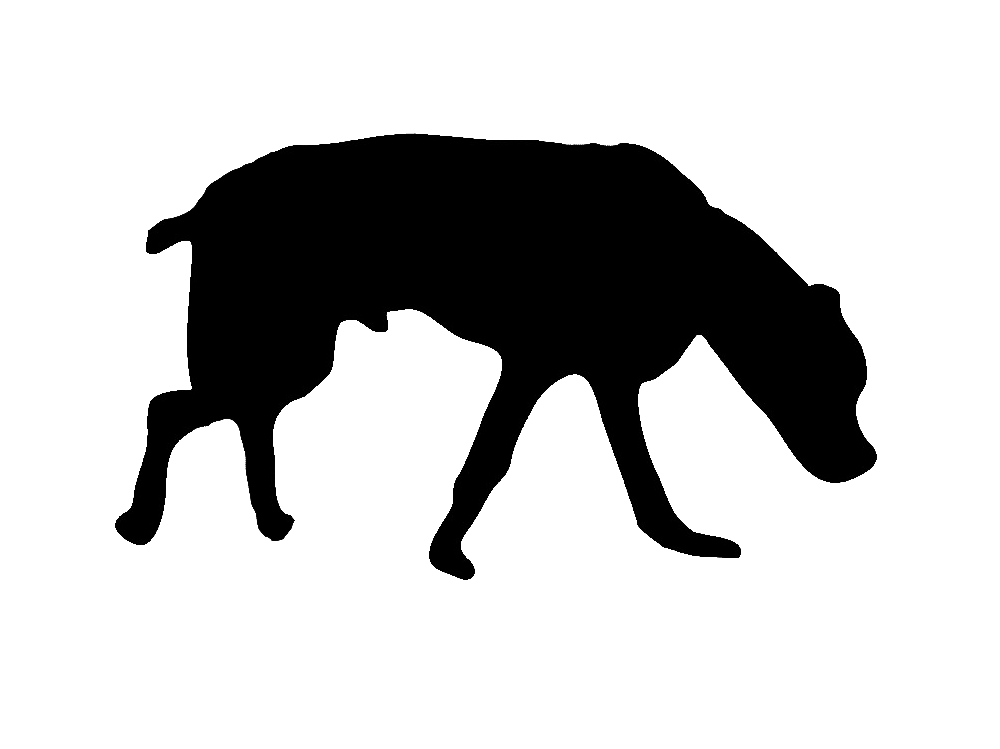
\includegraphics[scale=0.06]{img/dog}};
        \end{tikzpicture}
\end{column}
%\begin{column}{.5\linewidth}<3->
%    \begin{center}
%        \begin{tikzpicture}[overlay]
%            \node[yshift=-50] (img2) {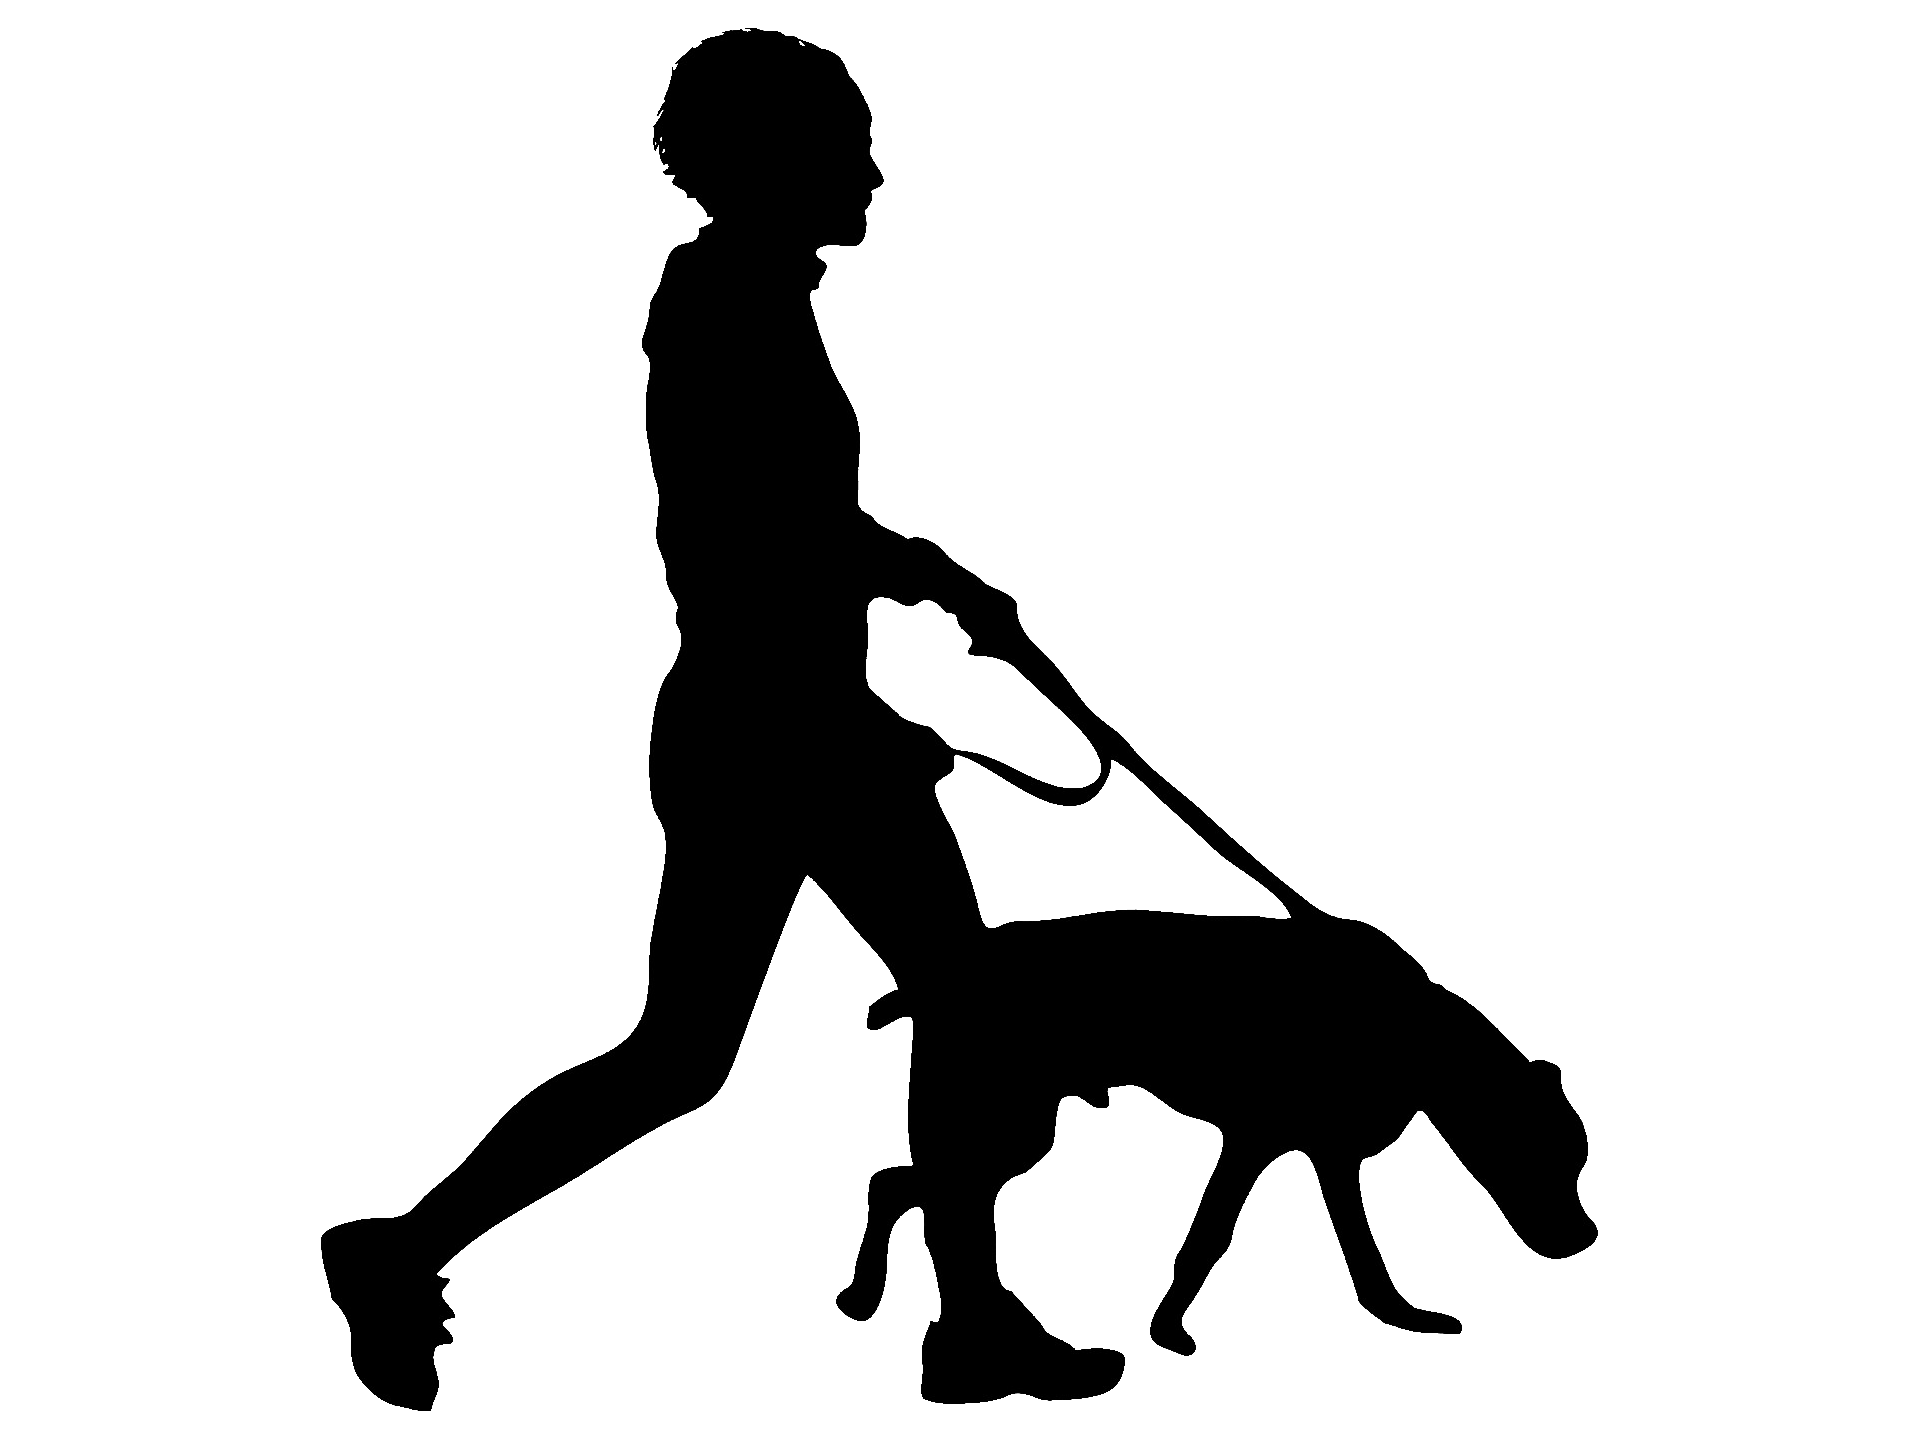
\includegraphics[scale=0.1]{img/mananddog}};
%        \end{tikzpicture}
%    \end{center}
%\end{column}
\end{columns}
\end{frame}


\begin{frame}[t,fragile]{Random walk and Cointegration Illustration}
 \begin{itemize}
  \item The drunk and dog's walk
 \end{itemize}
    \begin{center}
        \begin{tikzpicture}[overlay]
            \node[yshift=-60] (img2) {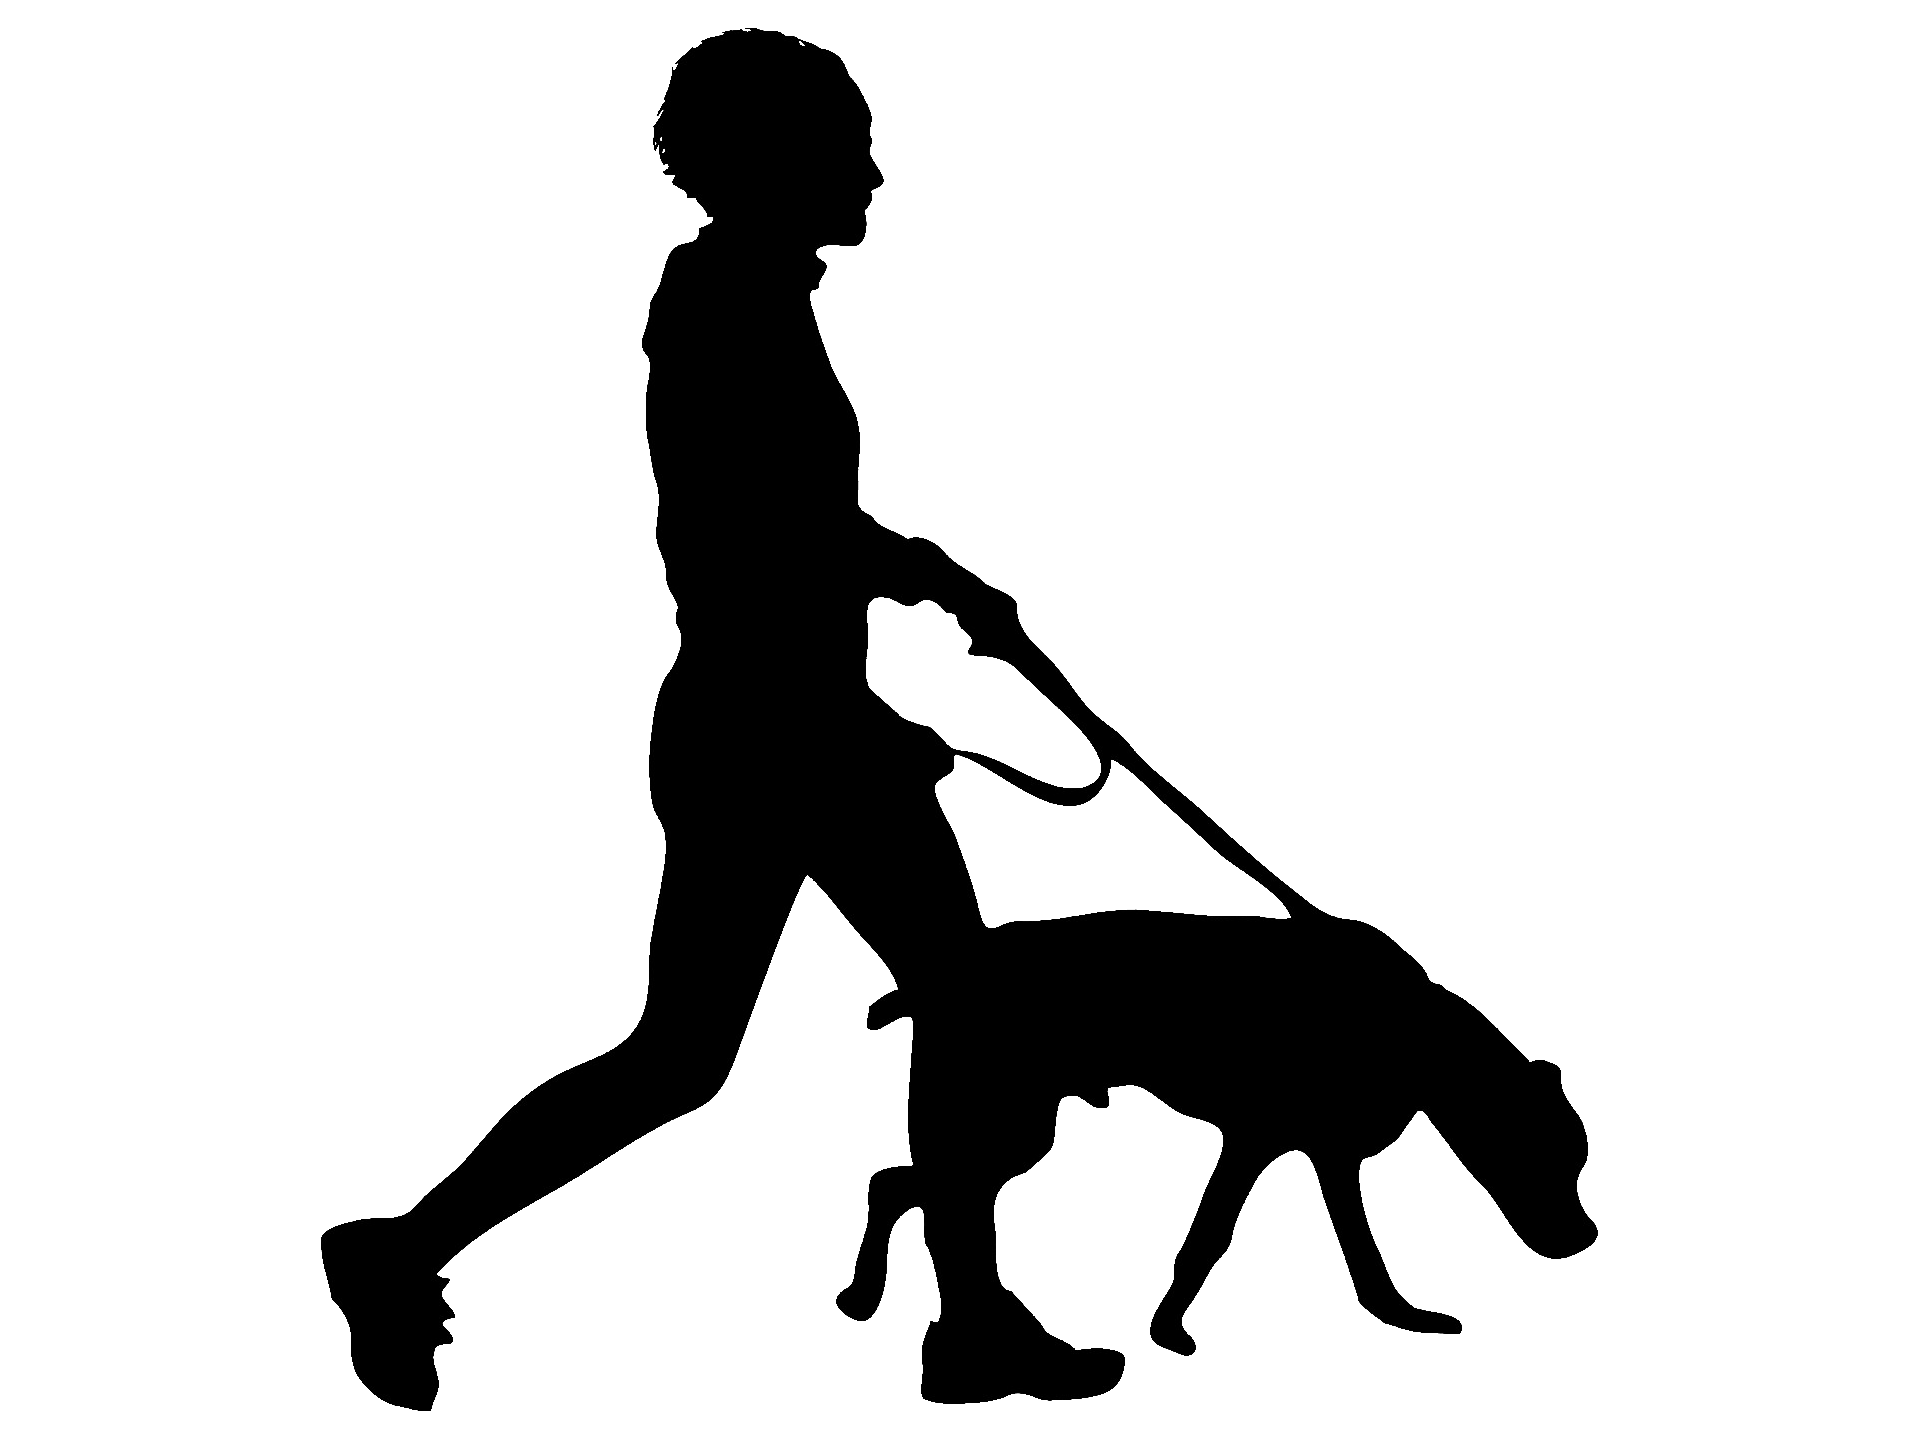
\includegraphics[scale=0.1]{img/mananddog}};
        \end{tikzpicture}
    \end{center}
\end{frame}


\begin{frame}
\frametitle{Motivation}

The relationship between non-stationary time series can be modelled if a stationary linear combination is shown to exist.
%Financial time series are mainly non-stationary.  However, one or more linear
%combinations of non-stationary time series can be stationary even though
%individually they are not. 
When this happens it is said they have a long-run
equilibrium relationship and the variables are {\color{red} cointegrated}.
\

\end{frame}

\tikzstyle{every picture}+=[remember picture]
\everymath{\displaystyle}
\begin{frame}
\frametitle{The Vector Error correction}
\tikzstyle{na} = [baseline=-.5ex]

The Vector Error correction model (VECM) is used to model cointegrated time series.

\Large
\begin{equation*}
 \Delta \mathbf{y}_t = \underbrace{
        \tikz[baseline]{
            \node[fill=red!20,ellipse,anchor=base] (t1)
            {$ \Omega\mathbf{y}_{t-1}$};
        }}_\text{Error correction term} +
        \underbrace{
        \tikz[baseline]{
            \node[fill=blue!20,anchor=base] (t2)
            {$\sum_{i=1}^{p-1} \phi_i^* \Delta \mathbf{y}_{t-i} $};
        }}_\text{Autorregresive term} +
        \underbrace{
        \tikz[baseline]{
            \node[fill=green!20,anchor=base] (t3)
            {$c$};
        }}_\text{Constant}
        +
        \underbrace{
        \tikz[baseline]{
            \node[fill=yellow!20,anchor=base] (t3)
            {$\mathbf{\epsilon}_t $};
        }}_\text{i.i.e}
\end{equation*}

\end{frame}


\begin{frame}
The Vector Error correction model (VECM) is used to model cointegrated time series but is used only with batch data and rarely used with high frequency data.
\end{frame}




\subsection{Proposal}
\begin{frame}
\frametitle{Proposal}
\begin{block}{}
To use VECM with high frequency data where the best parameters are updated when new data is available and do this is done in a fast way.
\end{block}
\end{frame}

%\section{Background}
%%
%%\begin{frame}
%%\frametitle{Integration }
%%\begin{block}{Integration of order $d$}
%%A time series $\mathbf{y}$ is said to be integrated of order $d$ if after
%%differentiating the variable $d$ times, we get an stationary process, more precisely:
%%\[
%%(1-L)^d \mathbf{y} \sim \text{I(0)} \, ,
%%\]
%%\noindent where I(0) is a stationary time series and $L$ is the lag operator:
%%\[
%%(1-L)\mathbf{y} = \Delta \mathbf{y}=\mathbf{y}_t  -\mathbf{y}_{t-1} \quad \forall t
%%\]
%%\end{block}
%%\end{frame}
%%
%%\subsection{Integration example}
%%\begin{frame}
%%\frametitle{Financial Time Series}
%%\begin{columns}
%%\column[t]{5cm}
%%High frequency financial time series are commonly an I(1) process 
%%\begin{center}
%%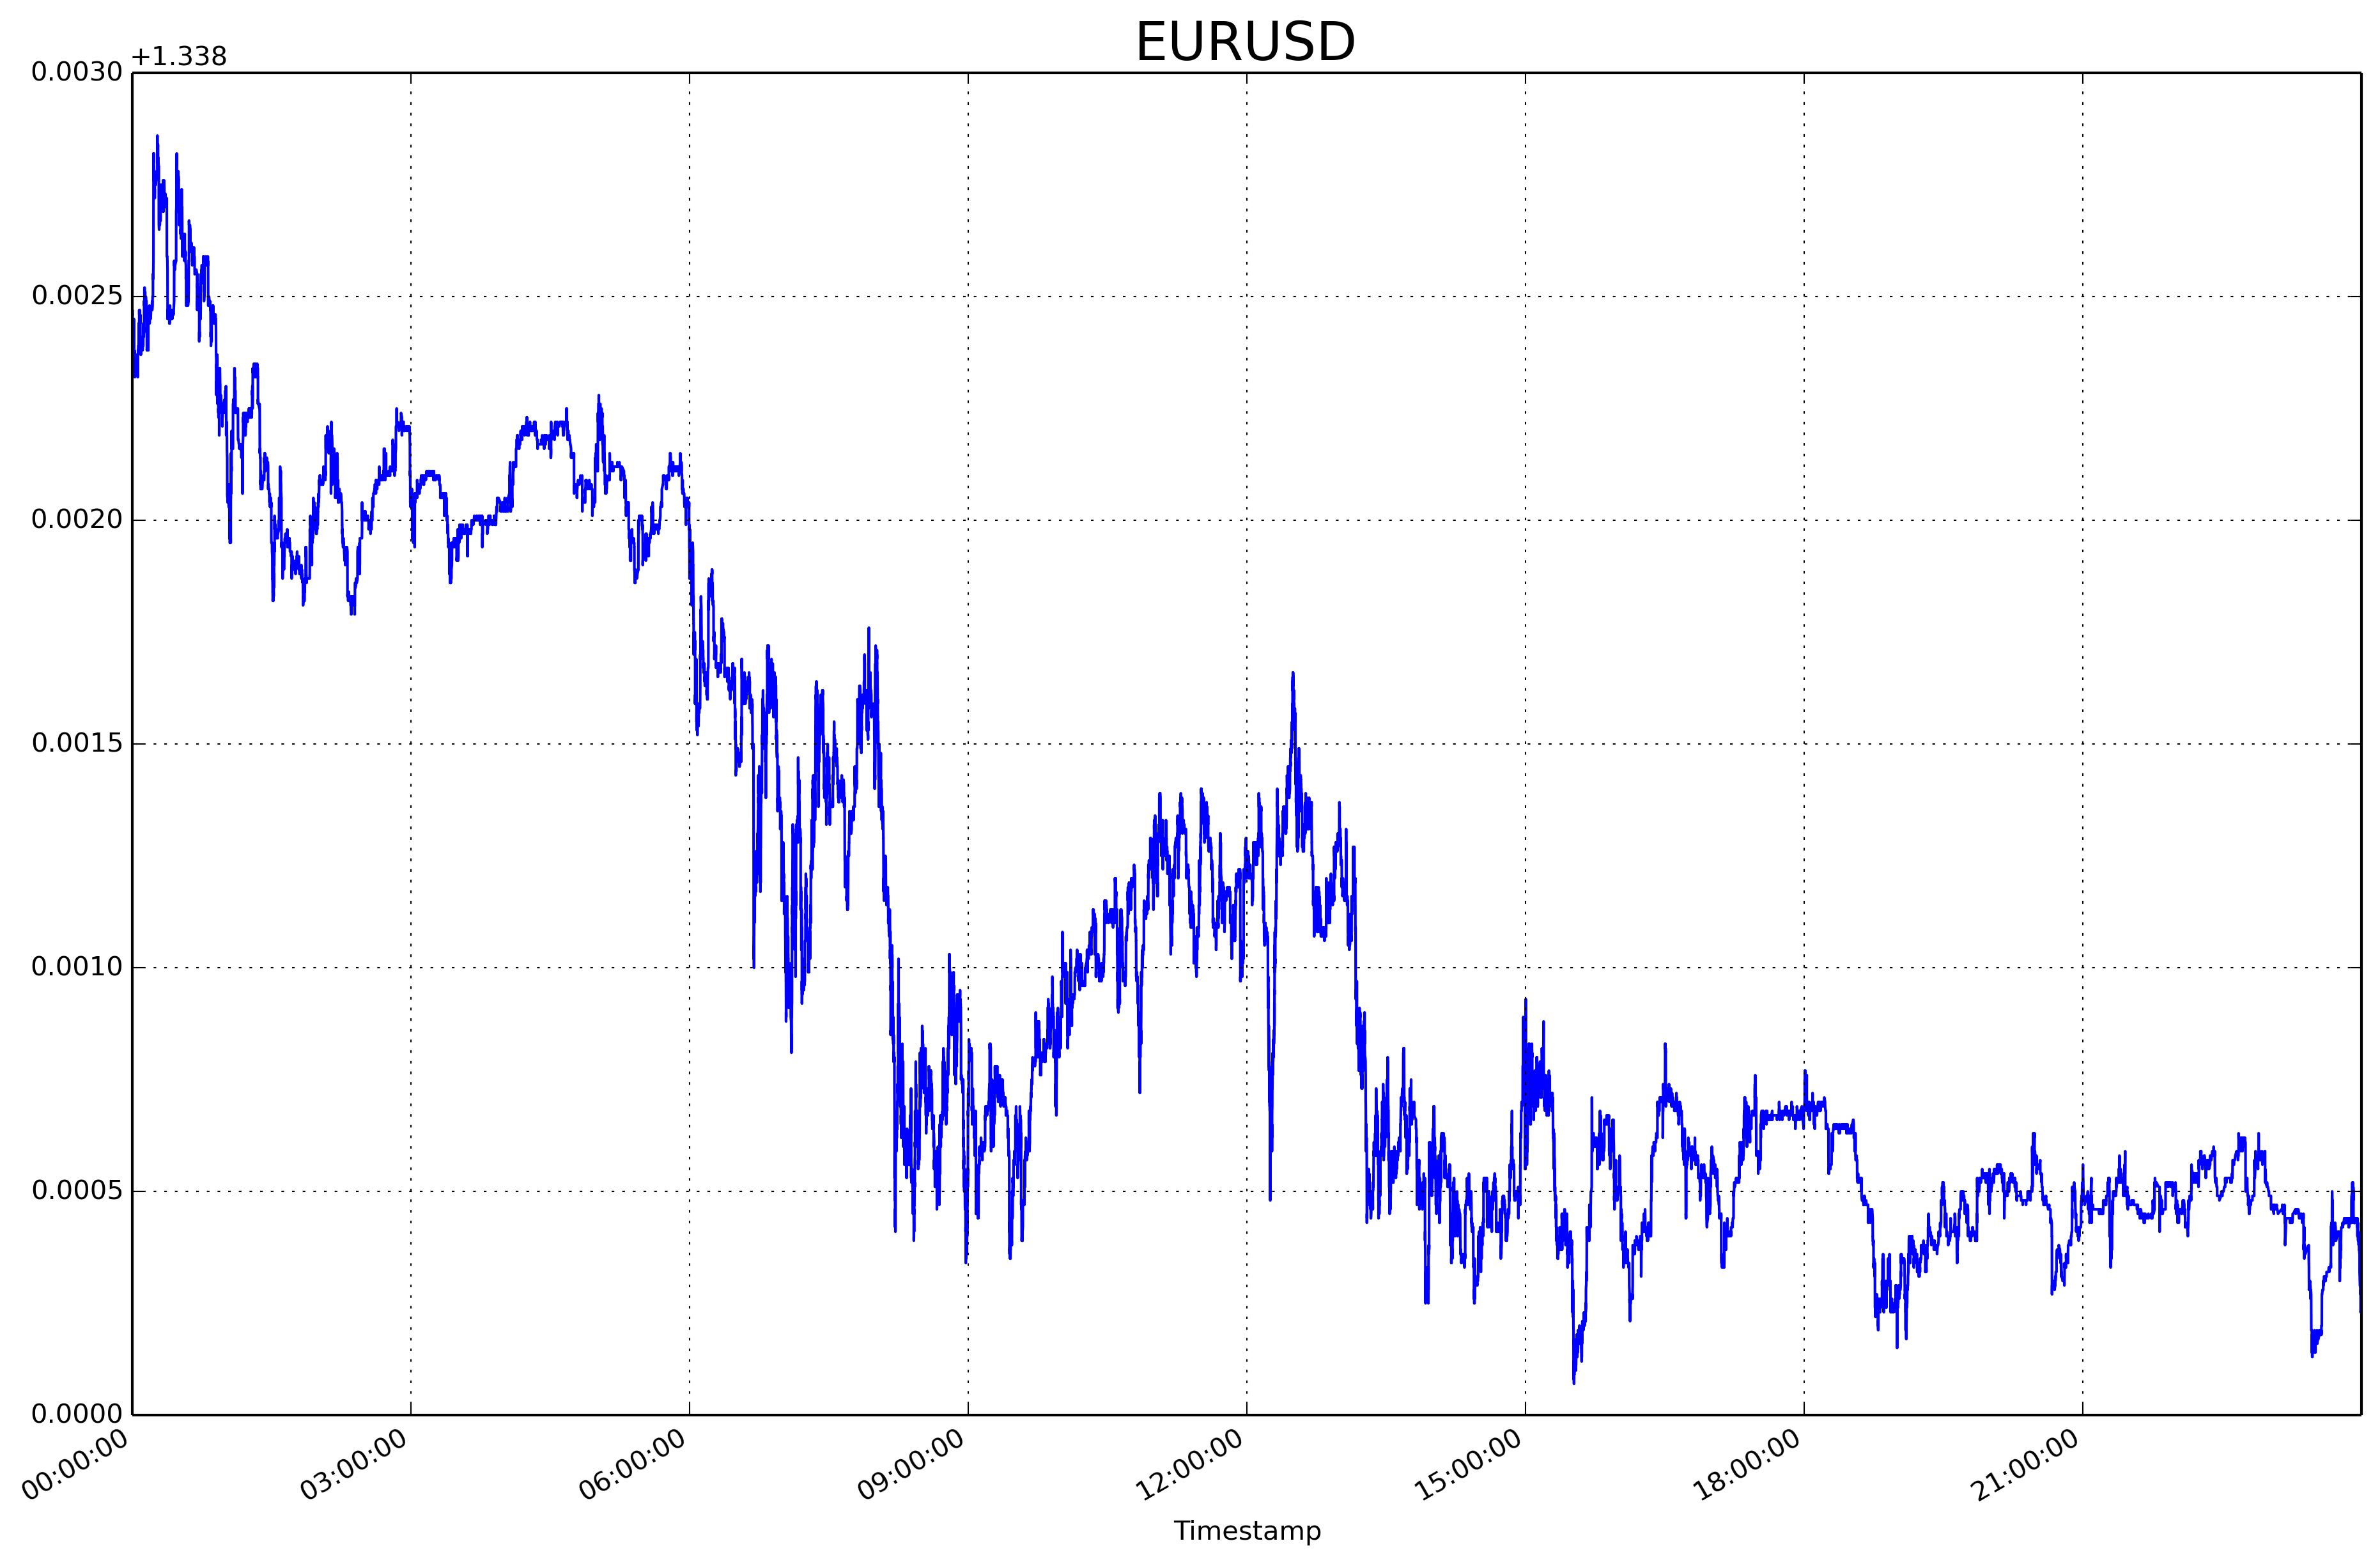
\includegraphics[width=0.85\textwidth]{img/EURUSD}
%%\end{center}
%%\column[t]{5cm}
%%Since their differences are stationary (I(0) process).
%%\begin{center}
%%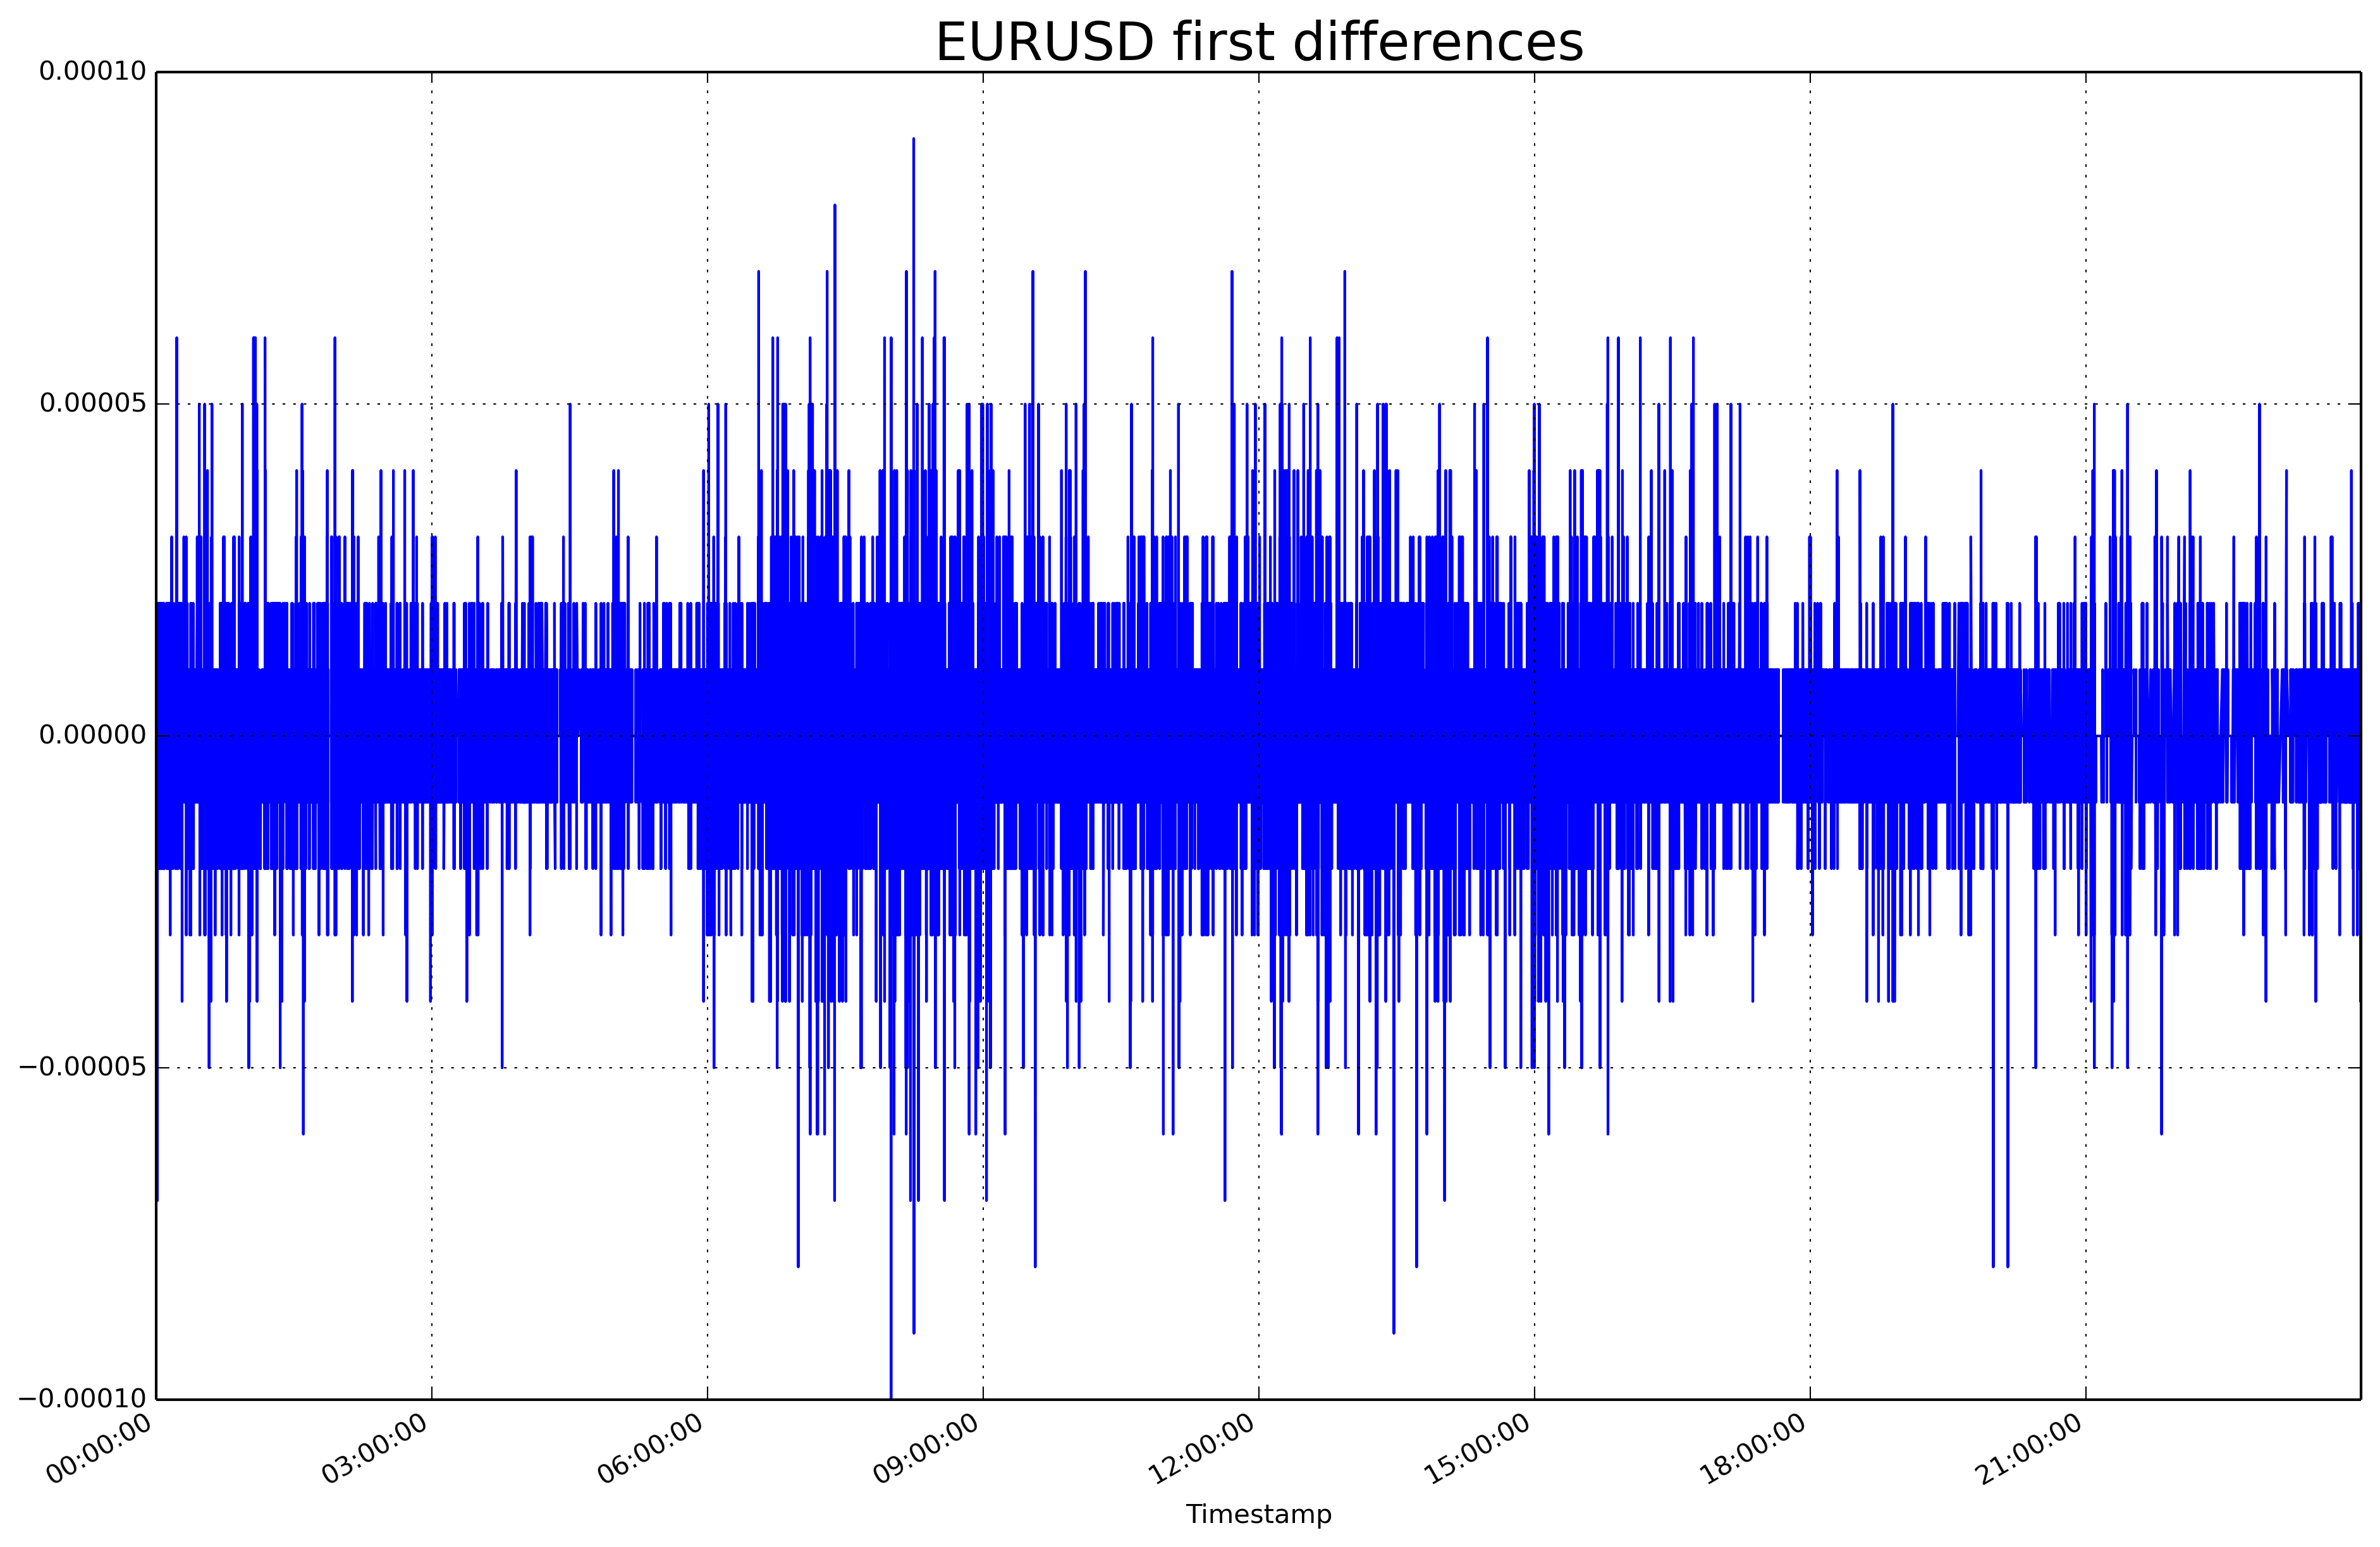
\includegraphics[width=0.85\textwidth]{img/DEURUSD}
%%\end{center}
%%\end{columns}
%%\end{frame}
%
%\subsection{Cointegration}
%\begin{frame}
%\frametitle{Cointegration}
%\begin{block}{Cointegration definition}
%Let $\mathbf{y} = \{\mathbf{y}^1, \dots, \mathbf{y}^l\}$ be a set of $l$
%time series of order I(1) which are said to be cointegrated if a vector
%$\beta=[\beta(1),\dots,\beta(l)]^\top \in \mathbb{R}^l$  exists such that the
%time series,
%
%\begin{equation*}
% \mathbf{Z}_t:= \beta^\top \mathbf{y} = \beta(1) \mathbf{y}^1 + \dots + \beta(l) \mathbf{y}^l \sim
% \text{I(0)}\, .
%\end{equation*}
%\end{block}
%In other words, a set of I(1) variables is said to be cointegrated if
%a linear combination of them exists which is I(0).
%
%\end{frame}
%
%\subsection{Vector Autorregresive models}
%\begin{frame}
%\frametitle{VECM: Vector Error Correction model}
%
%VECM is a special form of a Vector Autorregresive model (VAR) for I(1)
%variables $\mathbf{y}$ that are also cointegrated. Let 
%
%\begin{equation*}
%\label{eq:variables}
%\mathbf{y}_t = 
%\begin{bmatrix} y_{1,t} & y_{2,t} & \dots & y_{l,t}
%\end{bmatrix}^\top \, \qquad t=p+1, \dots N. 
%\end{equation*}
%
%\begin{block}{VAR}
%VAR($p$) model describes the behaviour of a set of $l$
%endogenous variables as a linear combination of their last $p$ values:
%{\color{blue}
%\begin{equation*}
%\label{eq:var}
% \mathbf{y}_t = \phi_1 \mathbf{y}_{t-1}  + \dots +   \phi_p\mathbf{y}_{t-p}
%+ \mathbf{c} + \mathbf{\epsilon}_t \, ,
%\end{equation*}}
%\noindent where  ${\phi_1,\dots,\phi_p}$ are $l \times l$
%matrices of real coefficients,
%$\mathbf{\epsilon}_{p+1},\dots,\mathbf{\epsilon}_N$ are error terms,
%$\mathbf{c}$ is a constant vector and $N$ is the total number of samples.
%\end{block}
%\end{frame}
%
%
%

%
%\noindent where 
%%coefficients matrices $\Omega$ and $\phi_i^*$ are
%%function of matrices $\phi_i$ as follows:
%
%\begin{eqnarray*}
%\phi_i^* &: =& -\sum_{j=i+1}^{p} \phi_j \\
%\Omega &: =& -(\mathbb{I}-\phi_1-\dots-\phi_p) 
%\end{eqnarray*}
%\end{frame}
%
%\begin{frame}
%\frametitle{$\Omega$ matrix properties}
%The matrix $\Omega$ has the following properties:
%\begin{itemize}
%\item If $\Omega = 0$ there is no cointegration
%\item If $rank(\Omega)=l$ i.e full rank, then the time series are not
%I(1) but stationary
%\item If $rank(\Omega)=r,\quad 0 < r < l$ then, there is cointegration
%and the matrix $\Omega$ can be expressed as $\Omega =
%\alpha \beta^\top$, where $\alpha$ and $\beta$ are $(l \times r)$
%matrices and $rank(\alpha)=rank(\beta)=r$.
%\end{itemize}
%The columns of $\beta$ contains the cointegration vectors and the rows of
%$\alpha$ correspond with the adjusted vectors. $\beta$ is obtained by Johansen
%procedure whereas $\alpha$ has to be determined as a
%variable in the VECM.
%\end{frame}
%
%
%\begin{frame}
%\frametitle{VECM matrix form}
%\small
%\begin{equation*}
%\underbrace{
%      \begin{bmatrix}
%       \mathbf{\Delta y}_{p+1}  \\ 
%       \mathbf{\Delta y}_{p+2}  \\ 
%       \vdots                   \\ 
%       \mathbf{\Delta y}_N      
%      \end{bmatrix}}_{\mathbf{B} } =
%\arraycolsep=1.4pt  
%\underbrace{\begin{bmatrix}
%   \alpha^\top & \phi^*_1 & \dots & \phi^*_{p-1} &\mathbf{c}   
%  \end{bmatrix}}_{\mathbf{X}^\top}
%\underbrace{\begin{bmatrix}
% \beta\mathbf{y}_p      & \beta\mathbf{y}_{p+1}   & \dots&   \beta\mathbf{y}_{N-1}   \\
% \mathbf{\Delta y}_{p}   & \mathbf{\Delta y}_{p+1}& \dots &  \mathbf{\Delta y}_{N-1} \\
% \mathbf{\Delta y}_{p-1} & \mathbf{\Delta y}_{p}  & \dots &  \mathbf{\Delta y}_{N-2}   \\
% \vdots                  & \vdots                 & \ddots&  \vdots                   \\
% \mathbf{\Delta y}_{2}   & \mathbf{\Delta y}_{3} & \dots &   \mathbf{\Delta y}_{N-p+1} \\
% 1                      & 1                       & \dots     & 1   
% \end{bmatrix}}_{\mathbf{A}^\top}
%+
%\underbrace{\begin{bmatrix}
%              \mathbf{\epsilon}_{p+1} \\ 
%              \mathbf{\epsilon}_{p+2} \\ 
%              \vdots \\ 
%              \mathbf{\epsilon}_N
%             \end{bmatrix}}_{\mathbf{E}^\top}
%\end{equation*}
%\end{frame}
%
%\section{Proposal}
%\subsection{Motivation}
%\begin{frame}
%\frametitle{VECM difficulties in an online context}
%\begin{itemize}
%\item VECM assumes cointegration vectors do not change in time. However, these might change due to several economic factors.
%\item To get updated cointegration vectors in time is computationally expensive because 
%the Johansen method and OLS are used to obtain them. It would be good to know how the number of cointegration vectors are affected by the number of data used $L$ and the number of lags of VECM $p$.
%\end{itemize}
%\end{frame}
%
%
%\begin{frame}
%\frametitle{Data}
%\begin{itemize}
%\item Tests were carried out using four foreign exchange rates all related to
%USD: EURUSD, GBPUSD, USDCHF and USDJPY. 
%\item This data was collected from Dukascopy, a free
%database which gives access to the Swiss Foreign Exchange marketplace.
%\item The tests were done using 10-seconds frequency from ask prices
%from the 11th to the 15th of August 2014. 
%%\item Since one day corresponds to 8640 data points and we used 5 days of data, we have 43,200 data points in total.
%\end{itemize}
%\end{frame}
%
%
%\begin{frame}
%\frametitle{Cointegration vectors distribution}
%\begin{figure}[!h]
%  %\vspace{-0.8cm}
%  \centering
%  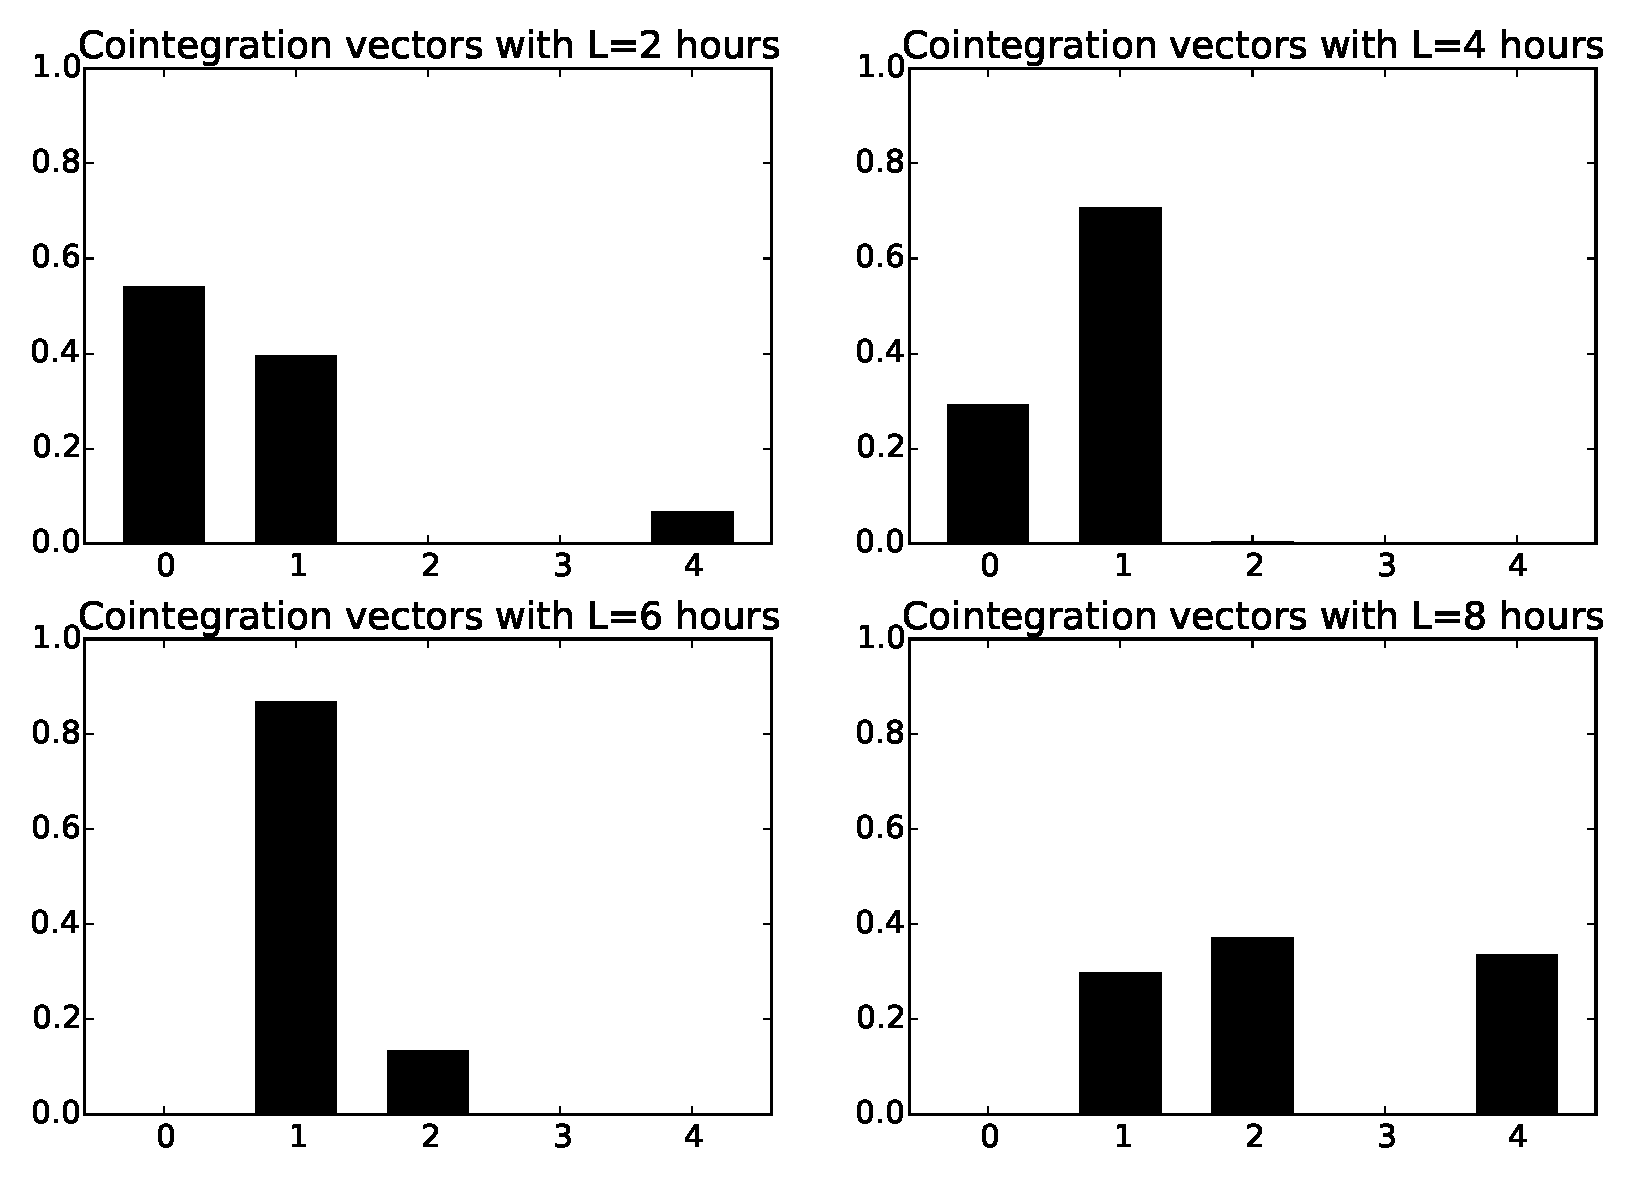
\includegraphics[width=0.75\textwidth]{img/histCointVectors-offset20520-p-1-freq-10s}
%  \caption{Histogram of the number of cointegration vectors using $p=1$. Four
%  possible values for $L$ are shown (100, 2000, 3000 and 4000).}
%  \label{fig:hists}
%\end{figure}
%\end{frame}
%
%\begin{frame}
%\frametitle{Percentage of cointegration}
%Since $r=0$ means no cointegration and $r=l=4$ reveals that no process is I(1) but stationary.
%The interesting cases of cointegration are those where $r$ lies strictly
%between $0$ and $l$, i.e. $0<r<l$.
%\begin{block}{Percentage of cointegration (PC)}
%{\color{blue}
%\begin{equation*} \label{eq:pcoint}
%PC = 
%\frac{\#\{ it \mid \text{$it$ has $r$ c.v. with $0<r<l$}\}}
%     {\#it}\times 100
%\end{equation*}}
%\end{block}
%\end{frame}
%
%
%\begin{frame}
%\frametitle{PC vs MSE}
%\begin{figure}[ht!]
%  %\vspace{-0.8cm}
%  \centering
%  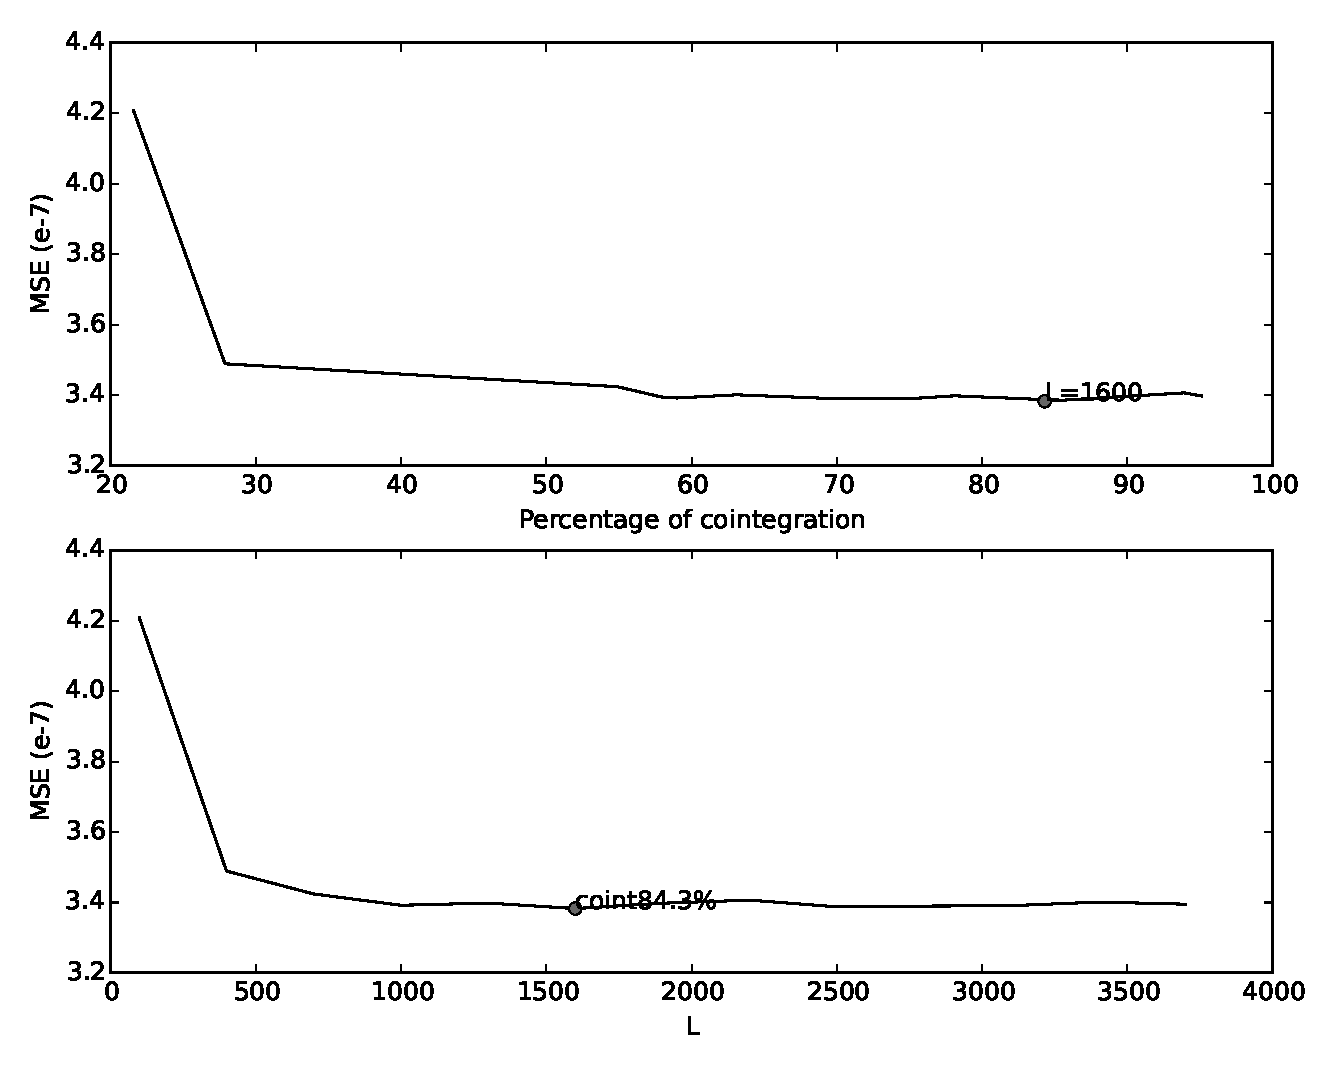
\includegraphics[width=0.7\textwidth]{img/MSE-offset20520-p-2-freq-10s}
%  \caption{MSE versus the percentage of cointegration considering 1000
%  iterations. }
%  \label{fig:cointvsmse}
%\end{figure}
%\end{frame}
%%%%%%%%%%%%%%%%%%%%%%%%%%%
%
%\subsection{AVECM}
%\begin{frame}
%\frametitle{Proposal: Adaptive VECM algorithm (AVECM)}
%\begin{itemize}
%\item We proposed to choose $L$ and $p$ in order to maximise the percentage of
%cointegration $PC$ in the near past. This process was done every time that new data was processed. 
%\item To use a distributed environment to make this parameters search, since this is the most expensive routine.
%\end{itemize}
%\end{frame}
%
%
%%\begin{frame}
%%\frametitle{AVECM Algorithm}
%%\begin{algorithmic}[1]
%%\REQUIRE $\,$ \\
%%$\mathbf{y}$: matrix with $N$ input vectors and $l$ time series\\
%%$j$: Starting point of testing \\
%%$it$: Ending point of testing \\
%%$ps$: list of $p$ values \\
%%$Ls$: list of $L$ values ($L<N$) \\
%%$m$: Iterations to determine parameters ($m < N-L$)\\
%%\ENSURE  $\,$ \\
%%$\{ \hat{\mathbf{y}}[1],\dots,\hat{\mathbf{y}}[it]\}$: prediction vectors \\
%%\FOR { $i =j$ to $it$ }
%%   \STATE $\mathbf{Y} \gets \mathbf{y}[:,i-1]$
%%    \STATE $L,p \gets
%%    \texttt{get\_best\_params}(Ls,ps,m,\mathbf{Y})$
%%        \STATE $model = \text{VECM}(\mathbf{Y},L, p)$
%%        \STATE $\hat{\mathbf{y}}[i-j] = model.predict()$
%%\ENDFOR
%%\end{algorithmic}
%%\end{frame}
%
%\subsection{Model comparison} 
%\begin{frame}
%\frametitle{Random walk}
%The random walk model is defined as:
%\begin{equation}
%\mathbf{y}_t = \mathbf{y}_{t-1} + \epsilon_{t}
%\label{rwmodel}
%\end{equation}
%The naive forecast of the time series difference $\hat{\mathbf{y}}_{t+1}$ for the random walk model is defined as:
%\begin{equation}
%\hat{\mathbf{y}}_{t+1} = \mathbf{y}_t + \hat{\epsilon}_{t+1} 
%\end{equation}
%\noindent where  $\hat{\epsilon}_{t+1} = \epsilon_{t}$.
%\end{frame}
%
%
%\begin{frame}
%\frametitle{ARIMA}
%A process can be modelled as an ARIMA$(p,d,q)$ if $\mathbf{x}_t = \Delta^d \mathbf{y}_t $, is an ARMA$(p,q)$. An ARMA$(p,q)$ model is the following:
%\begin{equation}
%\mathbf{x}_t = \sum_{i=1}^p \phi_i \mathbf{x}_{t-i}  +  \sum_{j=1}^q \theta_j \epsilon_{t-j}  
%\end{equation}
%\noindent with coefficients $\phi_p \neq 0$, $\theta_q \neq 0$ and $\sigma_{\epsilon}^2 > 0$.
%\end{frame}
%
%\begin{frame}
%\frametitle{Results}
%\begin{tabular}{ccccccc}
%
%& \multicolumn{3}{l}{MSE} & &
%\multicolumn{2}{c}{$U$-statistic} \\ 
%\hhline{~---~--} \\
% &
%AVECM & ARIMA & p-value & &
%AVECM & ARIMA \\ 
%
%\hline
% EURUSD & 1.07 e-09 & 1.14 e-09 &  9.25 e-12 & & 0.6863 & 0.7108\\
% GBPUSD & 1.66 e-09 & 1.74 e-09 &  6.95 e-02 & & 0.6866 & 0.7025\\
% USDCHF & 5.85 e-10 & 6.35 e-10 &  2.89 e-14 & & 0.6803 & 0.7091\\
% USDJPY  & 6.34 e-06 & 6.51 e-06 &  6.85 e-05 & & 0.6964 & 0.7057\\
% \end{tabular}
%\end{frame}
%
%%\begin{frame}
%%\frametitle{Evaluation methods}
%%\begin{block}{MSE}
%%Measures the distance between forecasts
%%and the true values and large deviations from the true value have a
%%large impact due to squaring forecast error.
%%{\color{blue}
%%\begin{equation}\label{eq:MSE}
%%\text{MSE} = 
%%\frac{\displaystyle \sum_{t=1}^{N} (\mathbf{y}_t-\hat{\mathbf{y}}_t)^2}{N}
%%\end{equation}}
%%\end{block}
%%\begin{block}{\bf $U$-statistic}
%%Unit free measure obtained as the ratio between the root MSE (RMSE) of a model and the RMSE of the naive random walk model. 
%%\end{block}
%%\end{frame}
%
%\section{Experiments}
%\subsection{Uno}
%
%%\begin{frame}
%%\frametitle{Unit root tests}
%%VECM can only be used if the time series are I(1). Therefore, 
%%before running the tests, we firstly checked whether the time series were
%%I(1) using the Augmented Dickey Fuller (ADF) test with lags $p=1,2,3,4,5$.
%%\end{frame}
%%
%%\begin{frame}
%%\frametitle{Performance accuracy}
%%\small
%%\begin{tabular}{ccccccc}
%%& \multicolumn{3}{l}{MSE} & &
%%\multicolumn{2}{c}{$U$-statistic} \\ 
%%\hhline{~---~--} \\
%% & AVECM & ARIMA & p-value & &
%%AVECM & ARIMA \\ 
%%
%%\hline
%% EURUSD & 1.0702 e-09 & 1.1481 e-09 &  9.250 e-12 & & 0.6863 & 0.7108\\
%% GBPUSD & 1.6630 e-09 & 1.7408 e-09 &  6.951 e-02 & & 0.6866 & 0.7025\\
%% USDCHF & 5.8503 e-10 & 6.3545 e-10 &  2.899 e-14 & & 0.6803 & 0.7091\\
%% USDJPY  & 6.3483 e-06 & 6.5194 e-06 &  6.853 e-05 & & 0.6964 & 0.7057
%% \end{tabular}
%% \end{frame}
%%For AVECM we considered different number of iterations (parameter $m$ in algorithm \ref{alg:AVECM}): 10, 50 and 100. We tried 12, 24 and 47 different pair of combinations for $L$ and $p$. Possible values for $L$ were in the interval $[100,4000]$ and $p$ can have values in between $[1,5]$. Best AVECM performance was compared against ARIMA and the random walk model.
%%Table~\ref{tab:stats} shows the out-of-sample performance measures: MSE and $U$-statistic for AVECM and ARIMA. In terms of both measures we found that AVECM is superior to ARIMA and the naive random walk model. We also included the p-value that proves that the difference in the MSE is significant at the 99\% significance level in three of the four currency rates and at 90\% in the case of GBPUSD. The $U$-statistic shows that AVECM and ARIMA are superior to the naive random walk model and that our proposal is also superior to ARIMA.
%
%
%
%\begin{frame}
%\frametitle{Parallel implementation}
%The function that get best parameters $L$ and $p$ was implemented using MPI in Python. MPI allows large-scale parallel applications
%with wide portability to be built, being able to run in large clusters
%or on local computers.
%We tested our proposal in a cluster with 2 servers Xeon E5-2667 (2.90GHz)
%of 24 cores each (48 cores in total) and 24GB RAM.
%\end{frame}
%
%\begin{frame}
%\frametitle{Parameters setting}
%\begin{itemize}
%%\item Parameter $it=100$
%\item The $L$ parameter was always chosen between 100 and 4000 and $p$ always took values
%between 1 and 5. 
%\item Parameter $nparams$ represents the number of pairs ($L$,$p$) used to maximise the percentage of cointegration. 
%\end{itemize}
%\end{frame}
%
%\begin{frame}
%\frametitle{Execution times}
%\begin{figure}[ht]
%  \centering
%  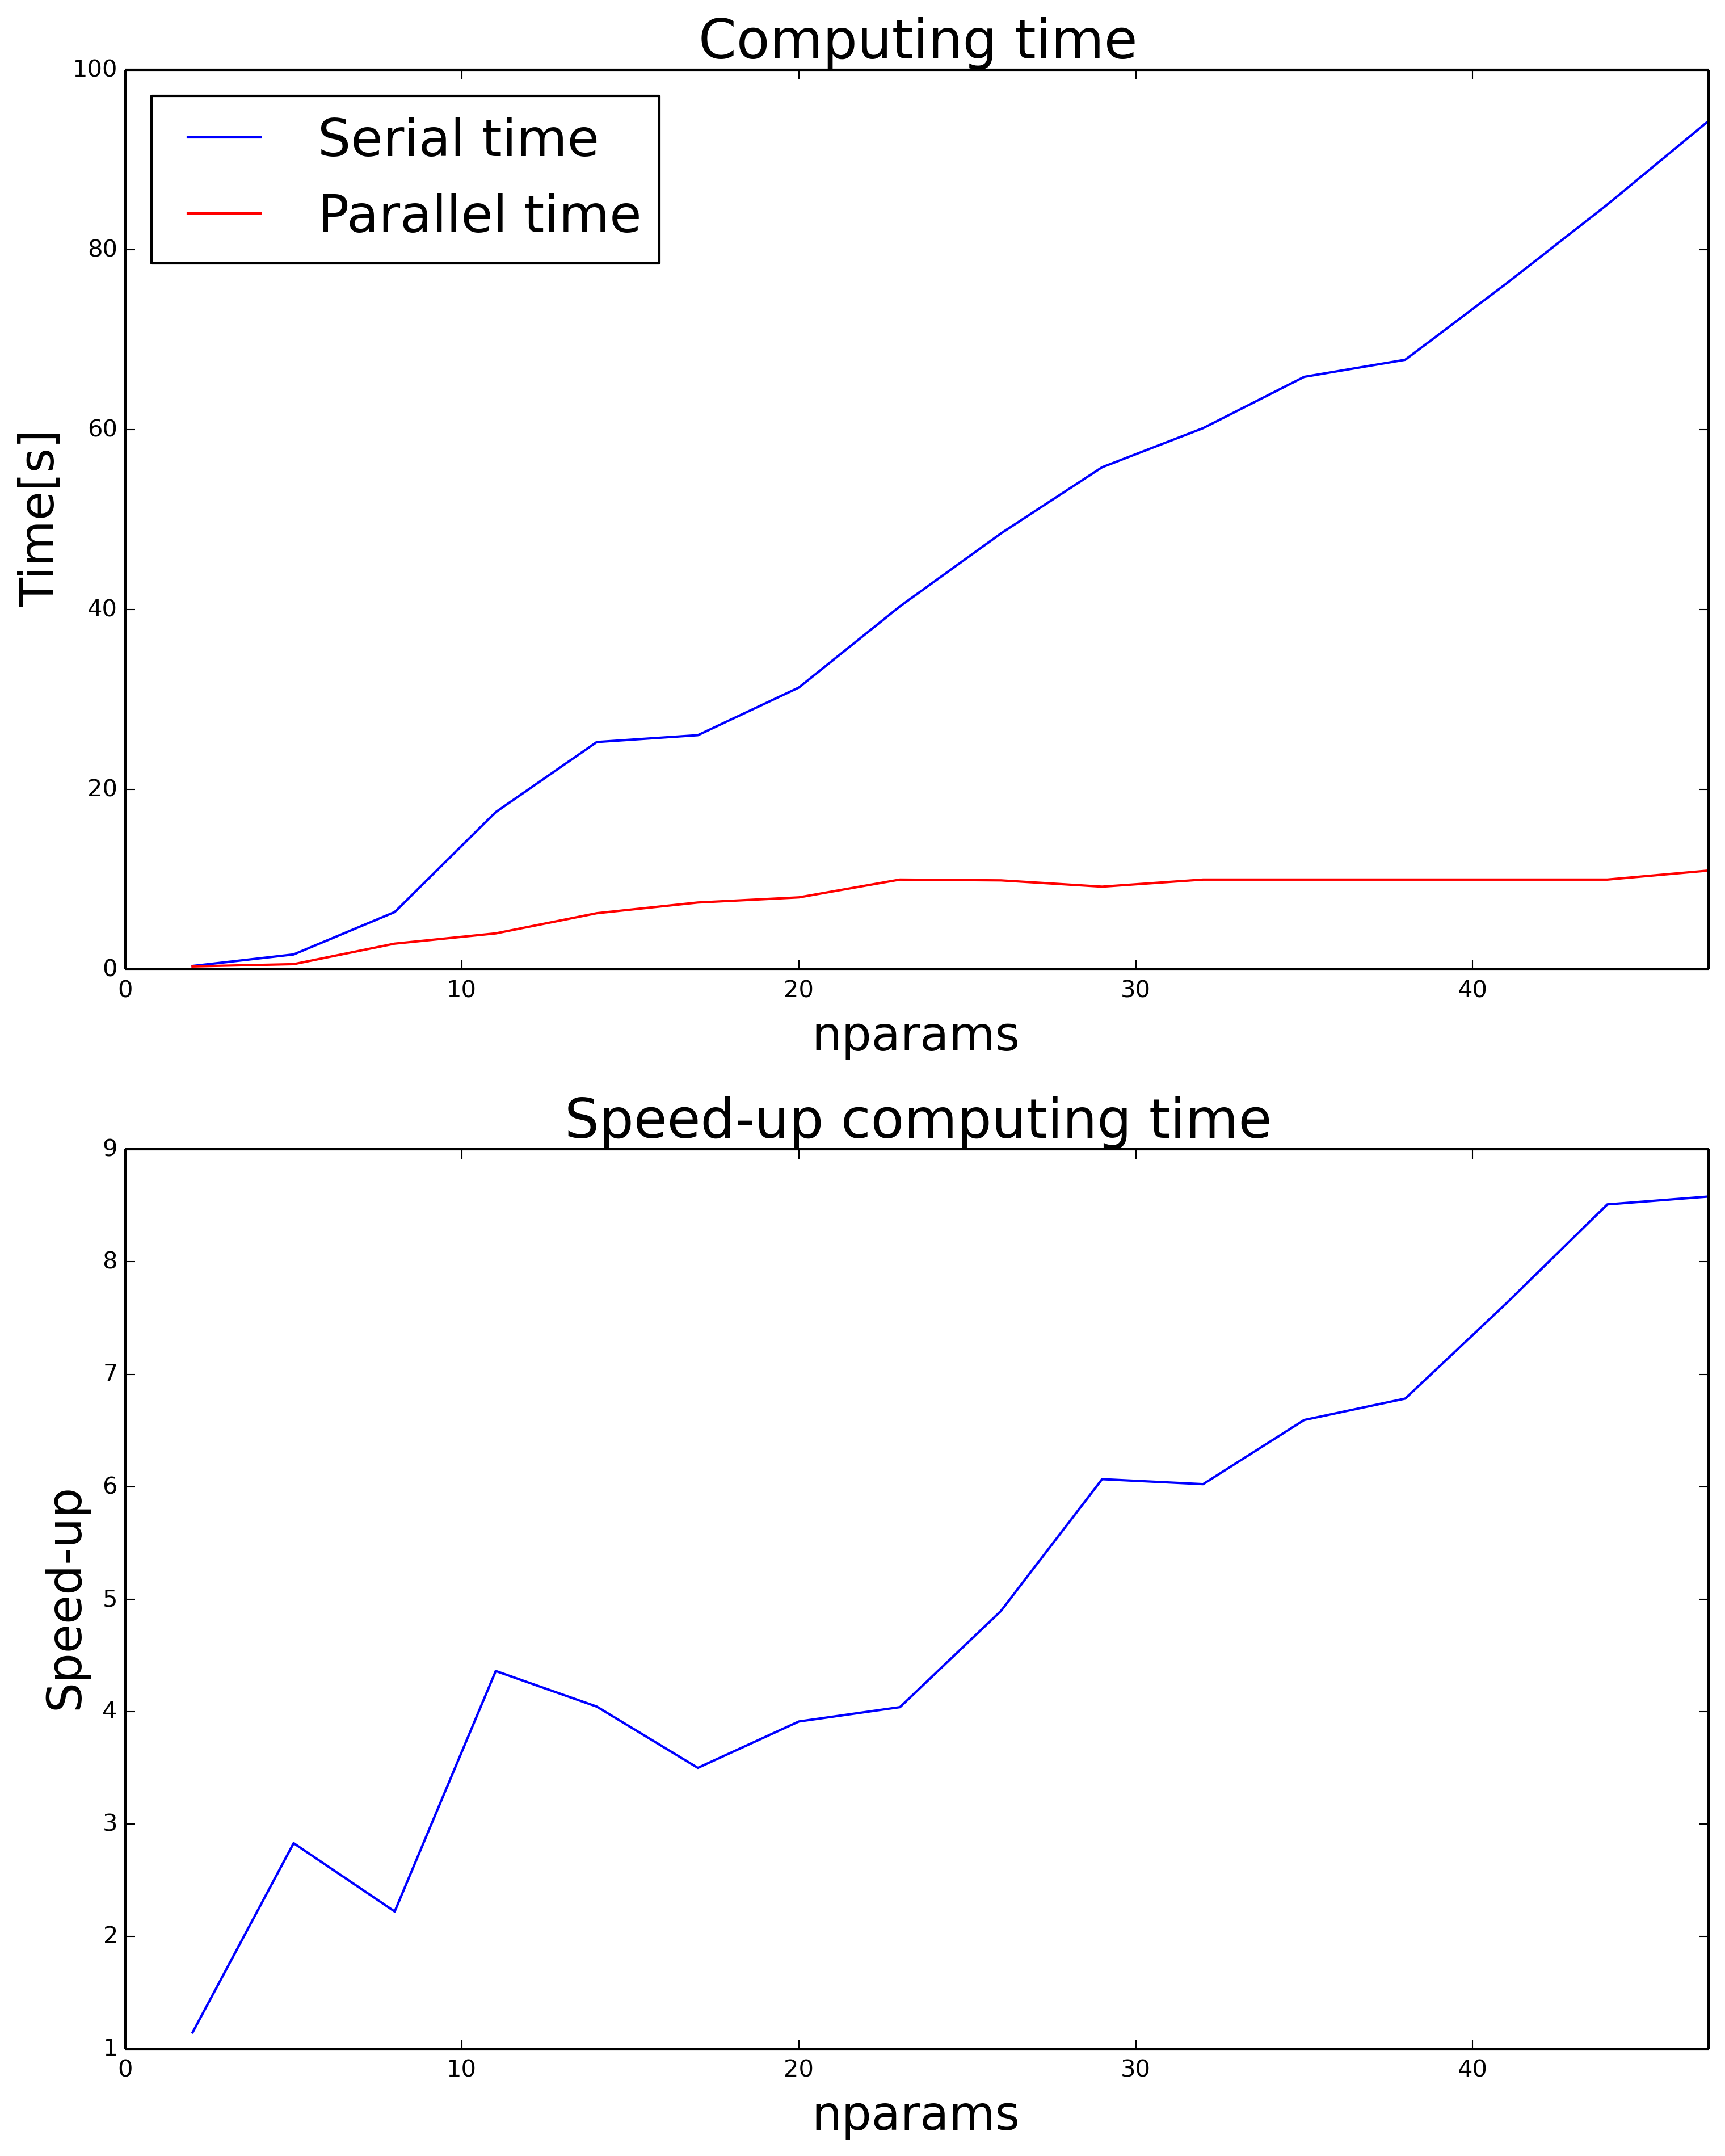
\includegraphics[width=0.75\textwidth]{img/extimes}
%  \caption{Computing time of sequential and parallel algorithm is shown in the
%  upper figure. Speed-up is shown below.}
%  \label{fig:extimes}
%% The superior figure \ref{fig:extimes} shows that best performance accuracy measurements are
%%achieved in times near or below 10 seconds in the parallel version. Contrarily,
%%serial times are high, above 10 seconds in most cases. Figure~\ref{fig:extimes} also shows the speed-up in computing time for AVECM which is near 9X if we use more than 25 parameters ($nparams$).
%%Execution times do not consider the loading data time, just that of finding
%%best parameters and matrix operations. The time MPI spends
%%transferring data and synchronising processes is about two seconds independently
%%of the number of processes considered. Execution times were measured using the Time python library.
%\end{figure}
%
%\end{frame}
%
%\section{Conclusions}
%\subsection{Uno}
%\begin{frame}
%\frametitle{Conclusions}
%\begin{itemize}
%\item Cointegration relations change with time. We empirically showed that the Johansen method is sensitive to the number of lags but also to the amount of data considered.
%\item We found that out-of-sample forecast performance MSE is related to the {\em percentage of cointegration\/}.  
%\item VECM improves performance measures by finding
%parameters of $L$ and $p$ maximising the percentage of cointegration.
%\item Increasing the number of parameters will always lead to
%better performance measures.
%\end{itemize}
%\end{frame}
%
%\begin{frame}
%\frametitle{Conclusions}
%\begin{itemize}
%\item The parallel implementation allowed the execution times to be reduced
%more than 9 times and therefore a response time was obtain before 10
%seconds. 
%\item For future study, it would be interesting to explore the relationship between
%cointegration and performance in order to propose new criteria for
%improving VECM parameters. It would also be interesting to include more 
%explaining variables such as bid-ask spread and change in volume.
%\end{itemize}
%\end{frame}

\begin{frame}[plain,c]
\begin{center}
\Huge Thank you for your attention
\Huge Questions?
\end{center}
\end{frame}
%Have a slide for each of the following
%9 Problem statement or Hypothesis
%9 “Why is this a Hard Problem?”
%9 Approach or Methodology
%9 “Why is this Innovative?”
%9 Assumptions and Constraints
%9 Initial Results (Promise of Great Things to Come)
%9 Validation Plan
%9 Limitations and Applicability
%9 Expected Contributions
%9 “What’s beyond this thesis?”
%9 Roadmap of Thesis



% Financial time series are not the only ones with this behaviour, this study can be extended to other non-stationary time series such as: weather, earthquakes, energy demand and sales forecasting.
\end{document}
